%%%% ijcai18.tex

\typeout{IJCAI-18 Instructions for Authors}

% These are the instructions for authors for IJCAI-18.
% They are the same as the ones for IJCAI-11 with superficical wording
%   changes only.

\documentclass{article}
\pdfpagewidth=8.5in
\pdfpageheight=11in
% The file ijcai18.sty is the style file for IJCAI-18 (same as ijcai08.sty).
\usepackage{ijcai18}

% Use the postscript times font!
\usepackage{times}
\usepackage{xcolor}
\usepackage{soul}
\usepackage[utf8]{inputenc}
\usepackage[small]{caption}

\usepackage{amsmath}
\usepackage{amssymb}
\usepackage{amsthm}
\usepackage{multirow}
\usepackage{tikz}
\usepackage{comment}

\newcommand{\tup}[1]{{\langle #1 \rangle}}

\newcommand{\pre}{\mathsf{pre}}     % precondition
\newcommand{\del}{\mathsf{del}}     % effect
\newcommand{\add}{\mathsf{add}}     % effect
\newcommand{\eff}{\mathsf{eff}}     % effect
\newcommand{\cond}{\mathsf{cond}}   % conditional effect
\newcommand{\true}{\mathsf{true}}   % true
\newcommand{\false}{\mathsf{false}} % false
\newcommand{\PE}{\mathrm{PE}}     % precondition
\newcommand{\strips}{\textsc{Strips}}     % strips

\newtheorem{theorem}{Theorem}
\newtheorem{lemma}[theorem]{Lemma}
\newtheorem{definition}[theorem]{Definition}

\usepackage{graphicx}
\usepackage{caption}
\usepackage{subcaption}
\usepackage{listings}
\usepackage{multicol}
\usepackage{arydshln}
\usetikzlibrary{calc,backgrounds,positioning,fit}

% the following package is optional:
%\usepackage{latexsym} 

% Following comment is from ijcai97-submit.tex:
% The preparation of these files was supported by Schlumberger Palo Alto
% Research, AT\&T Bell Laboratories, and Morgan Kaufmann Publishers.
% Shirley Jowell, of Morgan Kaufmann Publishers, and Peter F.
% Patel-Schneider, of AT\&T Bell Laboratories collaborated on their
% preparation.

% These instructions can be modified and used in other conferences as long
% as credit to the authors and supporting agencies is retained, this notice
% is not changed, and further modification or reuse is not restricted.
% Neither Shirley Jowell nor Peter F. Patel-Schneider can be listed as
% contacts for providing assistance without their prior permission.

% To use for other conferences, change references to files and the
% conference appropriate and use other authors, contacts, publishers, and
% organizations.
% Also change the deadline and address for returning papers and the length and
% page charge instructions.
% Put where the files are available in the appropriate places.

\title{Learning Strips Action Models from State-Constraints}

\author{Diego Aineto\and Sergio Jim\'enez\and Eva Onaindia\\
{\small Departamento de Sistemas Inform\'aticos y Computaci\'on}\\
{\small Universitat Polit\`ecnica de Val\`encia.}\\
{\small Camino de Vera s/n. 46022 Valencia, Spain}\\
{\small \{dieaigar,serjice,onaindia\}@dsic.upv.es}}

\begin{document}

\maketitle

\begin{abstract}
This paper presents a classical planning compilation for learning \strips\ action models from observations of plan executions. Interestingly the input to the compilation is a set of {\em state-constraints} that bounds the space of possible action models and that does not require the precise executed actions. The output is a possible action \strips\ action model, that satisfies the given state-constraints. Last but not least, the paper shows that our compilation is also extensible to include further information about the observed plan executions to increase the accuracy of the learned models.  
\end{abstract}

\section{Introduction}
Besides {\em plan synthesis}~\cite{ghallab2004automated}, planning action models are also useful for {\em plan/goal recognition}~\cite{ramirez2012plan}. At both planning tasks, an automated planner is required to reason about action models that correctly and completely capture the possible world transitions~\cite{geffner:book:2013}. Unfortunately, building planning action models is complex, even for planning experts, and this knowledge acquisition task is a bottleneck that limits the potential of AI planning~\cite{kambhampati:modellite:AAAI2007}.

Learning \strips\ action models from observations of plan executions is a well-studied problem with sophisticated algorithms, like {\sc ARMS}~\cite{yang2007learning}, {\sc SLAF}~\cite{amir:alearning:JAIR08} or {\sc LOCM}~\cite{cresswell2013acquiring}. Motivated by recent advances on the synthesis of different kinds of generative models with classical planning~\cite{bonet2009automatic,segovia2016hierarchical,segovia2017generating}, this paper introduces an innovative approach for learning \strips\ action models from observations of plan executions that:
\begin{enumerate}
\item Does not require information about the the precise applied actions.
\item Can be defined as a classical planning compilation which opens the door to the bootstrapping of planning action models.
\item Is extensible to include further information about the observed plan executions to increase the accuracy of the learned models.
\end{enumerate}


\section{Background}
This section defines the planning models used on this work and the output of the learning tasks addressed in the paper.

\subsection{Classical planning}
We use $F$ to denote the set of {\em fluents} (propositional variables) describing a state. A {\em literal} $l$ is a valuation of a fluent $f\in F$, i.e. either~$l=f$ or $l=\neg f$. A set of literals $L$ represents a partial assignment of values to fluents (WLOG we assume that $L$ does not assign conflicting values to any fluent). We use $\mathcal{L}(F)$ to denote the set of all literal sets on $F$, i.e.~all partial assignments of values to fluents.

A {\em state} $s$ is a full assignment of values to fluents, i.e. $|s|=|F|$, so the size of the state space is $2^{|F|}$. Explicitly including negative literals $\neg f$ in states simplifies subsequent definitions but often, we will abuse notation by defining a state $s$ only in terms of the fluents that are true in $s$, as is common in \strips\ planning.

A {\em classical planning frame} is a tuple $\Phi=\tup{F,A}$, where $F$ is a set of fluents and $A$ is a set of actions. Each action $a\in A$ comprises three sets of literals:
\begin{itemize}
\item $\pre(a)\subseteq\mathcal{L}(F)$, called {\em preconditions}, the literals that must hold for the action $a\in A$ to be applicable.
\item $\eff^+(a)\subseteq\mathcal{L}(F)$, called {\em positive effects}, that defines the fluents set to true by the application of the action $a\in A$.
\item $\eff^-(a)\subseteq\mathcal{L}(F)$, called {\em negative effects}, that defines the fluents set to false by the action application.
\end{itemize}
We say that an action $a\in A$ is {\em applicable} in a state $s$ iff $\pre(a)\subseteq s$. The result of applying $a$ in $s$ is the {\em successor state} $\theta(s,a)=\{s\setminus\eff^-(a))\cup\eff^+(a)\}$.

A {\em classical planning problem} is a tuple $P=\tup{F,A,I,G}$, where $I$ is an initial state and $G\subseteq\mathcal{L}(F)$ is a goal condition. A {\em plan} for $P$ is an action sequence $\pi=\tup{a_1, \ldots, a_n}$ that induces a state sequence $\tup{s_0, s_1, \ldots, s_n}$ such that $s_0=I$ and, for each {\small $1\leq i\leq n$}, $a_i$ is applicable in $s_{i-1}$ and generates the successor state $s_i=\theta(s_{i-1},a_i)$. We denote with $|\pi|$ the {\em plan length}. A plan $\pi$ {\em solves} $P$ iff $G\subseteq s_n$, i.e.~if the goal condition is satisfied at the last state reached after following the application of $\pi$ in $I$.


\subsection{Classical planning with conditional effects}
Our approach for learning \strips\ action models is compiling this leaning task into a classical planning task with conditional effects. Conditional effects allow us to compactly define actions whose effects depend on the current state. Supporting conditional effects is now a requirement of the IPC~\cite{vallati:IPC:AIM2015} and many classical planners cope with conditional effects without compiling them away.

An action $a\in A$ has now a set of {\em preconditions} $\pre(a)\in\mathcal{L}(F)$ and a set of {\em conditional effects} $\cond(a)$. Each conditional effect $C\rhd E\in\cond(a)$ is composed of two sets of literals $C\in\mathcal{L}(F)$, the {\em condition}, and $E\in\mathcal{L}(F)$, the {\em effect}.

An action $a\in A$ is {\em applicable} in a state $s$ if and only if $\pre(a)\subseteq s$, and the resulting set of {\em triggered effects} are the effects whose conditions hold in $s$:
\[
triggered(s,a)=\bigcup_{C\rhd E\in\cond(a),C\subseteq s} E,
\]

The result of applying an action $a$ in a state $s$ is the {\em successor} state $\theta(s,a)=\{s\setminus\eff_c^-(s,a))\cup\eff_c^+(s,a)\}$ where $\eff_c^-(s,a)\subseteq triggered(s,a)$ and $\eff_c^+(s,a)\subseteq triggered(s,a)$ are the triggered {\em negative} and {\em positive} effects, respectively.


\subsection{\strips\ action schemes and {\em variable name} objects}
This work addresses the learning of PDDL action schemes that follow the \strips\ requirement~\cite{mcdermott1998pddl,fox2003pddl2}. Figure~\ref{fig:stack} shows the schema, coded in PDDL, for the {\em stack} action from a four-operator {\em blocksworld}~\cite{slaney2001blocks}.

\begin{figure}
\begin{footnotesize}
\begin{verbatim}
(:action stack
  :parameters (?v1 ?v2 - object)
  :precondition (and (holding ?v1) (clear ?v2))
  :effect (and (not (holding ?v1))
               (not (clear ?v2))
               (handempty) (clear ?v1)
               (on ?v1 ?v2)))
\end{verbatim}
\end{footnotesize}
 \caption{\small \strips\ operator schema coding, in PDDL, the {\em stack} action from the {\em blocksworld}.}
\label{fig:stack}
\end{figure}

To formalize the output of the learning task, we assume that fluents $F$ are instantiated from a set of {\em predicates} $\Psi$, as in PDDL. Each predicate $p\in\Psi$ has an argument list of arity $ar(p)$. Given a set of {\em objects} $\Omega$, the set of fluents $F$ is induced by assigning objects in $\Omega$ to the arguments of predicates in $\Psi$, i.e.~$F=\{p(\omega):p\in\Psi,\omega\in\Omega^{ar(p)}\}$ s.t. $\Omega^k$ is the $k$-th Cartesian power of $\Omega$.

Let $\Omega_v=\{v_i\}_{i=1}^{\operatorname*{max}_{a\in A} ar(a)}$ be a new set of objects $\Omega\cap\Omega_v=\emptyset$, denoted as {\em variable names}, and that is bound by the maximum arity of an action in a given planning frame. For instance, in a three-block blocksworld $\Omega=\{block_1, block_2, block_3\}$ while $\Omega_v=\{v_1, v_2\}$ because the operators with the maximum arity, {\small\tt stack} and {\small\tt unstack}, have two parameters each.

Let us also define $F_v$, a new set of fluents $F\cap F_v=\emptyset$, that results from instantiating $\Psi$ using only the objects in $\Omega_v$ and that defines the elements that can appear in an action schema. For instance, in the blocksworld, $F_v$={\small\tt\{handempty, holding($v_1$), holding($v_2$), clear($v_1$), clear($v_2$), ontable($v_1$), ontable($v_2$), on($v_1,v_1$), on($v_1,v_2$), on($v_2,v_1$), on($v_2,v_2$)\}}.

Finally, we assume that actions $a\in A$ are instantiated from \strips\ operator schemes $\xi=\tup{head(\xi),pre(\xi),add(\xi),del(\xi)}$ where:
\begin{itemize}
\item $head(\xi)=\tup{name(\xi),pars(\xi)}$, is the operator {\em header} defined by its name and corresponding {\em variable names}, $pars(\xi)=\{v_i\}_{i=1}^{ar(\xi)}$. For instance, the headers for a four-operator blocksworld are: {\small\tt pickup($v_1$), putdown($v_1$), stack($v_1,v_2$)} and {\small\tt unstack($v_1,v_2$)}.
\item The preconditions $pre(\xi)\subseteq F_v$, the negative effects $del(\xi)\subseteq F_v$, and the positive effects $add(\xi)\subseteq F_v$ such that, $del(\xi)\subseteq pre(\xi)$, $del(\xi)\cap add(\xi)=\emptyset$ and $pre(\xi)\cap add(\xi)=\emptyset$.
\end{itemize}


\subsection{State-constraints}
A {\em state invariant} is a formula $\phi$ that holds in the initial state, formally $I\models \phi$, and at any state reachable from that state~\cite{rintanen:schematicInvariants:AAAI2017}, for all states $s$ reachable from $I$ $s\models \phi$.

A {\em mutex} is a particualr case of state invariant that take the form of a binary clause and that represents that a pair of different properties cannot be simultaneously true and are hence mutually exclusive. For instance, in a three-blocks blocksworld $on(block1,block2)$ and $on(block1,block3)$ are mutex.

A {\em domain invariant} is a particular state invariant that does not depend on a particular initial state, since they are instance-independent~\cite{kautz:mutex:IJCAI1999}. A {\em lifted invariant} is a state invariant defined usig a first order formula over the predicates of a given planning domain~\cite{rintanen:schematicInvariants:AAAI2017}. For instance in the blocksworld, $\forall x,y,z\ (on(x,y)\wedge on(x,z)) \implies y=z$, is a domain and lifted invariant because a block can only be on top of a single block no matter the initial state  and no matter the block.

Now we are ready to define a particular case of state-constraints called {\em lifted domain mutex} as a lifted domain invariant that takes the form of a binary clause. For instance, in the blocksworld $\forall x,y$ then $clear(x)$ and $on(x,y)$ is a {\em lifted domain mutex}.

{\em Linear Temporal Logic} (LTL) includes model operator that also allows to represent state constraints~\cite{haslum:LTL:ecai10}. For instance the {\em always} operator, denoted by $\square$, defines constraints that, like {\em lifted domain invariants}, must be true at any reachable state.


\section{Learning \strips\ action models}
Learning \strips\ action models from fully available input knowledge, i.e. from plans where the {\em pre-} and {\em post-states} of every action in a plan are available, is straightforward. When any intermediate state is available, \strips\ operator schemes are derived lifting the literals that change between the pre and post-state of the corresponding action executions. Preconditions are derived lifting the minimal set of literals that appears in all the pre-states of the corresponding actions.

This section formalizes more challenging learning tasks, where less input knowledge is available:

\subsubsection{Learning from state-constraints.} This learning task corresponds to observing an agent acting in the world but watching only the results of its plan executions. No information about the actions in the plans is given. This learning task is formalized as $\Lambda=\tup{\Psi,\Sigma,\Phi}$:
\begin{itemize}
\item $\Psi$ is the set of predicates that define the abstract state space of a given planning domain.
\item $\Sigma=\{\sigma_1,\ldots,\sigma_{\tau}\}$ is a set of state sequences $\sigma_t=(s_0^t,s_1^t,\ldots,s_{n}^t)$ such that,  {\small $1\leq i\leq n$} and {\tt\small $1\leq t\leq \tau$}, comprises the states resulting from executing an unknown plan $\pi_t$ starting from the {\em initial} state $s_0^t$.
\item $\Phi$ is a set of {\em lifted domain mutex}.
\end{itemize}

A solution to $\Lambda$ is a set of operator schema $\Xi$ that is compliant with the predicates in $\Psi$, the given set of states $\Sigma$ and the set of state constraints $\Phi$. In this learning scenario, a solution must not only determine a possible \strips\ action model but also the plans $\pi_t$, {\tt\small $1\leq t\leq \tau$} that explain the given set of states $\Sigma$ using the learned \strips\ model. 

\begin{figure}
{\tt ;;; Predicates in $\Psi$}
\begin{footnotesize}
\begin{verbatim}
(handempty) (holding ?o  - object)
(clear ?o - object) (ontable ?o - object)
(on ?o1 - object ?o2 - object)
\end{verbatim}
\end{footnotesize}

\vspace{0.2cm}

\begin{subfigure}{.6\textwidth}
{\tt ;;; Label $\sigma_1=(s_0^1,s_1^1,s_2^1,s_3^1)$}
\begin{lstlisting}[mathescape]
\end{lstlisting}
\vspace{0.1cm}
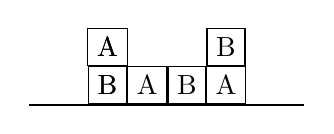
\begin{tikzpicture}[node distance = 0mm, block/.style args = {#1,#2}{fill=#1,text width=#2,shape=square}]
\node (initB) [draw, ]{B};
\node (initA) [draw, above=of initB.north]{A};
\node (twoB) [draw, right=of initB]{A};
\node (twoA) [draw, right=of twoB]{B};
\node (three) [draw, ]{B};
\node (three) [draw, above=of initB.north]{A};
\draw[thick] (-1,-0.25) -- (2.5,-0.25);
\node (goalB) [draw, right=10mm of initB]{A};
\node (goalA) [draw, right=10mm of initA]{B};
\end{tikzpicture}
\vspace{0.6cm}
\end{subfigure}%

\begin{subfigure}{.6\textwidth}
{\tt ;;; Label $\Phi$}
\begin{lstlisting}[mathescape]
(:derived (invariant-1-1)
  (forall (?o1 - object)
      (not (and (handempty) (holding ?o1)))))

(:derived (invariant-1-2)
  (forall (?o1 - object)
      (not (and (holding ?o1) (clear ?o1)))))

(:derived (invariant-1-3)
  (forall (?o1 - object)
      (not (and (holding ?o1) (ontable ?o1)))))

(:derived (invariant-1-4)
  (forall (?o1 - object)
      (not (and (on ?o1 ?o1)))))

;;;
;;; Invariants with two quantified variable and size 2
;;;
(:derived (invariant-2-1)
  (forall (?o1 ?o2 - object)
      (not (and (on ?o1 ?o2) (holding ?o1)))))

(:derived (invariant-2-2)
  (forall (?o1 ?o2 - object)
      (not (and (on ?o1 ?o2) (holding ?o2)))))

(:derived (invariant-2-3)
  (forall (?o1 ?o2 - object)
      (not (and (on ?o1 ?o2) (clear ?o2)))))

(:derived (invariant-2-4)
  (forall (?o1 ?o2 - object)
      (not (and (on ?o1 ?o2) (ontable ?o1)))))

(:derived (invariant-2-5)
  (forall (?o1 ?o2 - object)
      (not (and (on ?o1 ?o2) (on ?o2 ?o1)))))
\end{lstlisting}
\end{subfigure}%

 \caption{\small Example of a task for learning a \strips\ action model in the blocksworld from a single labeled plan.}
\label{fig:lexample}
\end{figure}


\section{Learning \strips\ action models with planning}
Our approach for addressing the learning task $\Lambda$, is compiling it into a classical planning task with conditional effects. The intuition behind the compilation is that a solution to the resulting classical planning task is a sequence of actions that:
\begin{enumerate}
\item Programs the \strips\ action model $\Xi$. A solution plan has a {\em prefix} that, for each $\xi\in\Xi$, determines the fluents from $F_v$ that belong to its $pre(\xi)$, $del(\xi)$ and $add(\xi)$ sets.
\item Validates the programmed \strips\ action model $\Xi$ in the given input knowledge (the sequences of states $\Sigma$, and $\Phi$ if available). For every $\sigma_t\in \Sigma$, a solution plan has a postfix that produces a final state $s_{n}^t$ starting from the corresponding initial state $s_0^t$ using the programmed action model $\Xi$. We call this process the validation of the programmed \strips\ action model $\Xi$, at the learning example {\small $1\leq t\leq \tau$}. %If information about the corresponding plan $\pi_t\in \Pi$ is available, then it is also used in the validation.
\end{enumerate}

To formalize our compilation we first define {\small $1\leq t\leq \tau$} classical planning instances $P_t=\tup{F,\emptyset,I_t,G_t}$ that belong to the same planning frame (i.e. same fluents and actions but differ in the initial state and goals). Fluents $F$ are built instantiating the predicates in $\Psi$ with the objects appearing in the input labels $\Sigma$. Formally $\Omega=\{o|o\in \bigcup_{\small 1\leq t\leq \tau} obj(s_0^t)\}$, where $obj$ is a function that returns the set of objects that appear in a fully specified state. The set of actions, $A=\emptyset$, is empty because the action model is initially unknown. Finally, the initial state $I_t$ is given by the state $s_0^t\in \sigma_t$ while goals $G_t$, are defined by the state $s_n^t\in \sigma_t$.

Now we are ready to formalize the compilations. We start with $\Lambda$, because it requires less input knowledge. Given a learning task $\Lambda=\tup{\Psi,\Sigma}$ the compilation outputs a classical planning task $P_{\Lambda}=\tup{F_{\Lambda},A_{\Lambda},I_{\Lambda},G_{\Lambda}}$:
\begin{itemize}
\item $F_{\Lambda}$ extends $F$ with:
\begin{itemize}
\item Fluents representing the programmed action model $pre_f(\xi)$, $del_f(\xi)$ and $add_f(\xi)$, for every $f\in F_v$ and $\xi \in \Xi$. If a fluent $pre_f(\xi)/del_f(\xi)/add_f(\xi)$ holds, it means that $f$ is a precondition/negative effect/positive effect in the \strips\ operator schema $\xi\in \Xi$. For instance, the preconditions of the $stack$ schema (Figure~\ref{fig:stack}) are represented by fluents {\small\tt pre\_holding\_stack\_$v_1$} and {\small\tt pre\_clear\_stack\_$v_2$}.
\item A fluent $mode_{prog}$ indicating whether the operator schemes are being programmed or validated (already programmed) and fluents $\{test_t\}_{1\leq t\leq \tau}$, indicating the example where the action model is being validated.
\end{itemize}
\item $I_{\Lambda}$ contains the fluents from $F$ that encode $s_0^1$ (the initial state of the first label), every $pre_f(\xi)\in F_{\Lambda}$ and $mode_{prog}$ set to true. Our compilation assumes that initially any operator schema is programmed with every possible precondition, no negative effect and no positive effect.
\item $G_{\Lambda}=\bigcup_{1\leq t\leq \tau}\{test_t\}$, indicates that the programmed action model is validated in all the learning examples.
\item $A_{\Lambda}$ contains actions of three kinds:
\begin{enumerate}
\item Actions for {\em programming} an operator schema $\xi\in\Xi$:
\begin{itemize}
\item Actions for {\bf removing} a {\em precondition} $f\in F_v$ from the action schema $\xi\in\Xi$.

\begin{small}
\begin{align*}
\hspace*{7pt}\pre(\mathsf{programPre_{f,\xi}})=&\{\neg del_{f}(\xi),\neg add_{f}(\xi),\\
& mode_{prog}, pre_{f}(\xi)\},\\
\cond(\mathsf{programPre_{f,\xi}})=&\{\emptyset\}\rhd\{\neg pre_{f}(\xi)\}.
\end{align*}
\end{small}

\item Actions for {\bf adding} a {\em negative} or {\em positive} effect $f\in F_v$ to the action schema $\xi\in\Xi$.

\begin{small}
\begin{align*}
\hspace*{7pt}\pre(\mathsf{programEff_{f,\xi}})=&\{\neg del_{f}(\xi),\neg add_{f}(\xi),\\
& mode_{prog}\},\\
\cond(\mathsf{programEff_{f,\xi}})=&\{pre_{f}(\xi)\}\rhd\{del_{f}(\xi)\},\\
&\{\neg pre_{f}(\xi)\}\rhd\{add_{f}(\xi)\}.
\end{align*}
\end{small}
\end{itemize}

\item Actions for {\em applying} an already programmed operator schema $\xi\in\Xi$ bound with the objects $\omega\subseteq\Omega^{ar(\xi)}$. We assume operators headers are known so the binding of the operator schema is done implicitly by order of appearance of the action parameters, i.e. variables $pars(\xi)$ are bound to the objects in $\omega$ appearing at the same position. 
\begin{small}
\begin{align*}
\hspace*{7pt}\pre(\mathsf{apply_{\xi,\omega}})=&\{pre_{f}(\xi)\implies p(\omega)\}_{\forall p\in\Psi,f=p(pars(\xi))},\\
\cond(\mathsf{apply_{\xi,\omega}})=&\{del_{f}(\xi)\}\rhd\{\neg p(\omega)\}_{\forall p\in\Psi,f=p(pars(\xi))},\\
&\{add_{f}(\xi)\}\rhd\{p(\omega)\}_{\forall p\in\Psi,f=p(pars(\xi))},\\
&\{mode_{prog}\}\rhd\{\neg mode_{prog}\}.
\end{align*}
\end{small}

\item Actions for {\em validating} the learning example {\tt\small $1\leq t\leq \tau$}.
\begin{small}
\begin{align*}
\hspace*{7pt}\pre(\mathsf{validate_{t}})=&G_t\cup\{test_j\}_{j\in 1\leq j<t}\\
&\cup\{\neg test_j\}_{j\in t\leq j\leq \tau}\cup \{\neg mode_{prog}\},\\
\cond(\mathsf{validate_{t}})=&\{\emptyset\}\rhd\{test_t\}.
\end{align*}
\end{small}
\end{enumerate}
\end{itemize}

\begin{lemma}
Any classical plan $\pi$ that solves $P_{\Lambda}$ induces an action model $\Xi$ that solves the learning task $\Lambda$.
\end{lemma}

\begin{proof}[Proof sketch]
\begin{small}
The compilation forces that once the preconditions of an operator schema $\xi \in \Xi$ are programmed, they cannot be altered. The same happens with the positive and negative effects that define an operator schema $\xi \in \Xi$ (besides they can only be programmed after preconditions are programmed). Once operator schemes are programmed they can only be applied because of the $mode_{prog}$ fluent. To solve $P_{\Lambda}$, goals $\{test_t\}$, {\small $1\leq t\leq \tau$} can only be achieved: executing an applicable sequence of programmed operator schemes that reaches the final state $s_n^t$, defined in $\sigma_t$, starting from $s_0^t$. If this is achieved for all the input examples {\small $1\leq t\leq \tau$}, it means that the programmed action model $\Xi$ is compliant with the provided input knowledge and hence, it is a solution to $\Lambda$.
\end{small}
\end{proof}

The compilation is {\em complete} in the sense that it does not discard any possible \strips\ action model.


\section{Constraining the learning hypothesis space with additional input knowledge}
\label{sec:Constraining}
Here we show that further input knowledge can be used to constrain the space of possible action models and make the learning of \strips\ action models more practicable.

\subsection{State-constraints}

\subsection{Plan constraints}
\subsubsection{Learning from labeled plans.}
Here we augment the input knowledge with the actions executed by the observed agent.

\begin{itemize}
\item $\Pi=\{\pi_1,\ldots,\pi_{\tau}\}$ is a given set of example plans where each plan $\pi_t=\tup{a_1^t, \ldots, a_n^t}$, {\small $1\leq t\leq \tau$}, is an action sequence that induces the corresponding state sequence $\tup{s_0^t, s_1^t, \ldots, s_n^t}$ such that, for each {\small $1\leq i\leq n$}, $a_i^t$ is applicable in $s_{i-1}^t$ and generates $s_i^t=\theta(s_{i-1}^t,a_i^t)$.
\end{itemize}

We extend the compilation to consider labeled plans. Given a learning task $\Lambda'=\tup{\Psi,\Sigma,\Pi}$, the compilation outputs a classical planning task $P_{\Lambda'}=\tup{F_{\Lambda'},A_{\Lambda'},I_{\Lambda'},G_{\Lambda'}}$ that extends $P_{\Lambda}$ as follows:
\begin{itemize}
\item $F_{\Lambda'}$ extends $F_{\Lambda}$ with $F_{\Pi}=\{plan(name(\xi),\Omega^{ar(\xi)},j)\}$, the fluents to code the steps of the plans in $\Pi$, where $F_{\pi_t}\subseteq F_{\Pi}$ encodes $\pi_t\in \Pi$. Fluents $at_j$ and $next_{j,j_2}$, {\small $1\leq j<j2\leq n$}, are also added to represent the current plan step and to iterate through the steps of a plan.
\item $I_{\Lambda'}$ extends $I_{\Lambda}$ with fluents $F_{\pi_1}$ plus fluents $at_1$ and $\{next_{j,j_2}\}$, {\small $1\leq j<j2\leq n$}, for indicating the plan step where the action model is validated. Goals are $G_{\Lambda'}=G_{\Lambda}=\bigcup_{1\leq t\leq \tau}\{test_t\}$, as in the original compilation.
\item With respect to $A_{\Lambda'}$.
\begin{enumerate}
\item The actions for {\em programming} the preconditions/effects of a given operator schema $\xi\in\Xi$ are the same.
\item The actions for {\em applying} an already programmed operator have an extra precondition $f\in F_{\Pi}$, that encodes the current plan step, and extra conditional effects $\{at_{j}\}\rhd\{\neg at_{j},at_{j+1}\}_{\forall j\in [1,n]}$ for advancing to the next plan step. This mechanism forces that these actions are only applied as in the example plans.
\item The actions for {\em validating} the current learning example have an extra precondition, $at_{|\pi_t|}$, to indicate that the current plan $\pi_t$ was fully executed and extra conditional effects to unload plan $\pi_{t}$ and load the next plan $\pi_{t+1}$:
\begin{small}
\begin{align*}
&\{\emptyset\}\rhd\{\neg at_{|\pi_t|},at_1\}, \{f\}\rhd\{\neg f\}_{f\in F_{\pi_t}}, \{\emptyset\}\rhd\{f\}_{f\in F_{\pi_t+1}}.
\end{align*}
\end{small}
\end{enumerate}
\end{itemize}


\section{Evaluation}
This section evaluates the performance of our approach for learning \strips\ action models starting from different amounts of available input knowledge.

\subsubsection{Setup.}
The domains used in the evaluation are IPC domains that satisfy the \strips\ requirement~\cite{fox2003pddl2}, taken from the {\sc planning.domains} repository~\cite{muise2016planning}. We only use 5 learning examples for each domain and they are fixed for all the experiments so we can evaluate the impact of the input knowledge in the quality of the learned models. All experiments are run on an Intel Core i5 3.10 GHz x 4 with 4 GB of RAM.

\subsubsection{Reproducibility.}
We make fully available the compilation source code, the evaluation scripts and the used benchmarks at this anonymous repository {\em https://github.com/anonsub/strips-learning} so any experimental data reported in the paper is fully reproducible. 

\subsubsection{Planner.}
The classical planner we use to solve the instances that result from our compilations is {\sc Madagascar}~\cite{rintanen2014madagascar}. We use {\sc Madagascar} because its ability to deal with planning instances populated with dead-ends. In addition, SAT-based planners can apply the actions for programming preconditions in a single planning step (in parallel) because these actions do not interact. Actions for programming action effects can also be applied in a single planning step reducing significantly the planning horizon.

\subsubsection{Metrics.}
The quality of the learned models is quantified with the {\em precision} and {\em recall} metrics. Intuitively, precision gives a notion of {\em soundness} while recall gives a notion of the {\em completeness} of the learned models. Formally, $Precision=\frac{tp}{tp+fp}$, where $tp$ is the number of true positives (predicates that correctly appear in the action model) and $fp$ is the number of false positives (predicates appear in the learned action model that should not appear). Recall is formally defined as $Recall=\frac{tp}{tp+fn}$ where $fn$ is the number of false negatives (predicates that should appear in the learned action model but are missing).


\section{Conclusions}

\newpage

%% The file named.bst is a bibliography style file for BibTeX 0.99c
\bibliographystyle{named}
\bibliography{constraints-learning}

\end{document}

